\section{Podstawy ruchu}

\begin{frame}{Globalne współrzędne -- Kula (Układ Sferyczny)}
    Zanim dron poleci, musi wiedzieć gdzie jest na Ziemi. Najprostszym modelem jest \textbf{kula}. Pozycję określamy za pomocą długości i szerokości geograficznej oraz promienia.
    
    \vspace{0.2cm}
    \begin{center}
    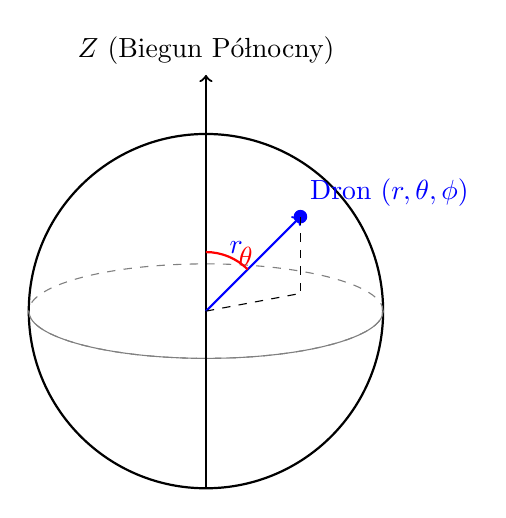
\begin{tikzpicture}[scale=1.5]
        % Sfera
        \draw[thick] (0,0) circle (1.5cm);
        \draw[dashed, gray] (0,0) ellipse (1.5cm and 0.4cm); % Równik tył
        \draw[gray] (-1.5,0) arc (180:360:1.5cm and 0.4cm);  % Równik przód
        
        % Oś Z
        \draw[->, thick] (0,-1.5) -- (0,2) node[anchor=south]{$Z$ (Biegun Północny)};
        
        % Punkt
        \filldraw[blue] (0.8, 0.8) circle (1.5pt) node[anchor=south west]{Dron $(r, \theta, \phi)$};
        \draw[->, thick, blue] (0,0) -- (0.8, 0.8) node[midway, above left]{$r$};
        
        % Rzuty
        \draw[dashed] (0.8, 0.8) -- (0.8, 0.15);
        \draw[dashed] (0,0) -- (0.8, 0.15);
        
        % Kąty
        \draw[red, thick] (0,0.5) arc (90:45:0.5cm) node[midway, right]{$\theta$};
    \end{tikzpicture}
    \end{center}
\end{frame}

\begin{frame}{Czy Ziemia to idealna kula? -- Układ Elipsoidalny}
    Ziemia jest spłaszczona na biegunach. W systemach GPS (np. standardzie WGS84) dron korzysta z \textbf{elipsoidy obrotowej}. 
    
    \vspace{0.2cm}
    \begin{center}
    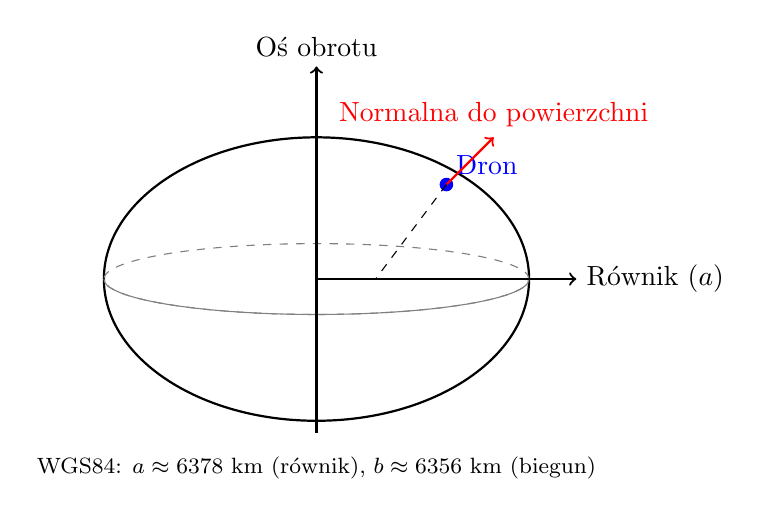
\begin{tikzpicture}[scale=1.5]
        % Elipsoida
        \draw[thick] (0,0) ellipse (1.8cm and 1.2cm);
        \draw[dashed, gray] (0,0) ellipse (1.8cm and 0.3cm); 
        \draw[gray] (-1.8,0) arc (180:360:1.8cm and 0.3cm); 
        
        % Osie
        \draw[->, thick] (0,-1.3) -- (0,1.8) node[anchor=south]{Oś obrotu};
        \draw[->, thick] (0,0) -- (2.2,0) node[anchor=west]{Równik ($a$)};
        
        % Punkt i normalna
        \filldraw[blue] (1.1, 0.8) circle (1.5pt) node[anchor=south west]{Dron};
        \draw[->, red, thick] (1.1, 0.8) -- (1.5, 1.2) node[anchor=south]{Normalna do powierzchni};
        \draw[dashed] (1.1, 0.8) -- (0.5, 0);
        
        \node[font=\footnotesize] at (0, -1.6) {WGS84: $a \approx 6378$ km (równik), $b \approx 6356$ km (biegun)};
    \end{tikzpicture}
    \end{center}
\end{frame}

\begin{frame}{Gdy jesteśmy blisko celu -- Układ lokalny NED}
    Globalne współrzędne (GPS) mają dziwne stopnie i radiany. Dla wygody obliczeń, wokół drona tworzy się płaski układ lokalny \textbf{NED} (North-East-Down).
    
    \vspace{0.2cm}
    \begin{center}
    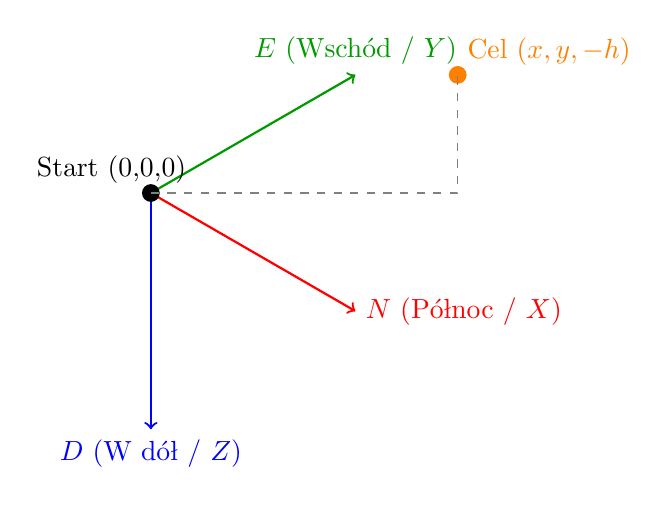
\begin{tikzpicture}[scale=1.5, x={(0.866cm, -0.5cm)}, y={(0.866cm, 0.5cm)}, z={(0cm, -1cm)}]
        % Osie NED (Z skierowane w dół!)
        \draw[->, thick, red] (0,0,0) -- (2,0,0) node[anchor=west]{$N$ (Północ / $X$)};
        \draw[->, thick, green!60!black] (0,0,0) -- (0,2,0) node[anchor=south]{$E$ (Wschód / $Y$)};
        \draw[->, thick, blue] (0,0,0) -- (0,0,2) node[anchor=north]{$D$ (W dół / $Z$)};
        
        % Dron
        \filldraw[black] (0,0,0) circle (2pt) node[anchor=south, xshift=-0.5cm]{Start (0,0,0)};
        \filldraw[orange] (1.5, 1.5, -1) circle (2pt) node[anchor=south west]{Cel $(x, y, -h)$};
        
        \draw[dashed, gray] (0,0,0) -- (1.5, 1.5, 0) -- (1.5, 1.5, -1);
    \end{tikzpicture}
    \end{center}
\end{frame}

\begin{frame}{Start drona -- pierwszy kod}
    Korzystając z lokalnego układu NED, polecamy maszynie polecieć 10 metrów na Północ i 5 metrów w Górę ($D = -5$).
    
    \vspace{0.5cm}
    \textbf{Demonstracja wideo:} Start i lot po prostej trajektorii.
    
    \begin{center}
    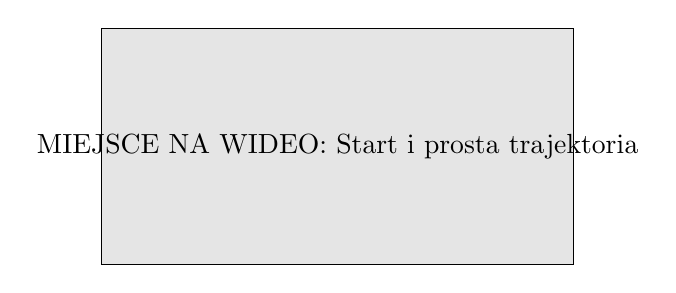
\begin{tikzpicture}
        \draw[fill=gray!20] (0,0) rectangle (6,3);
        \node at (3,1.5) {MIEJSCE NA WIDEO: Start i prosta trajektoria};
    \end{tikzpicture}
    \end{center}
\end{frame}
